\pdfoutput=1
\documentclass[twocolumn]{aastex61}
%%\documentclass[]{emulateapj}

%Accepted/received/... %%

\received{xxx}
\revised{yyy}
\accepted{zzz}

%% Command to document which AAS Journal the manuscript was submitted to.
\submitjournal{AAS Journals}

%% Short title/authors

\shorttitle{Tidal Torques in Stellar Binaries}
\shortauthors{Fleming et al.}

%% Begin document, title, packages %%
\usepackage{hyperref}
\usepackage{xspace}
\usepackage{graphicx}
\usepackage{amsmath}
\usepackage[caption=false]{subfig}

%% Custom commands
\def\mearth{{\rm\,M_\oplus}}
\def\rearth{{\rm\,R_\oplus}}
\def\msun{{\rm\,M_\odot}}
\def\rsun{{\rm\,R_\odot}}
\def\lsun{{\rm\,L_\odot}}
\def\gsim{~\rlap{$>$}{\lower 1.0ex\hbox{$\sim$}}}
\def\lsim{~\rlap{$<$}{\lower 1.0ex\hbox{$\sim$}}}

\newcommand{\vplanet}[0]{\texttt{VPLanet}\xspace}
\newcommand{\eqtide}[0]{\texttt{EQTIDE}\xspace}
\newcommand{\stellar}[0]{\texttt{STELLAR}\xspace}
\newcommand{\kepler}[0]{\textit{Kepler}\xspace}


%% Begin doc %%

\begin{document}

\title{Rotation Periods in Low-Mass Binary Stars: The Impact of Tidal Torques}

%% AUTHORS %%

%%\correspondingauthor{David P. Fleming}
%%\email{dflemin3@uw.edu}

%%\author[0000-0001-9293-4043]{David P. Fleming}
\author{David P. Fleming et al}
\affil{Astronomy Department, University of Washington \\
Box 951580, Seattle, WA 98195}

%% ABSTRACT %%

\begin{abstract}

- 5 points with Porb < 10 days and Porb/Prot > 10 in lurie plot are likely young stars that have or continue to spin up via angular momentum conservation due to pre main sequence contraction.  evidence for young stars in the Kepler field, e.g. McQuillan+2014, Matt+2015, Davenport+2017,2018 support this theory

- Lurie finds tons of short Porb EBs because transit observational biases favor bodies with short orbital periods for a finite observing window, eg Kepler's lifetime 

- Consult Lurie's paper for CPL vs CTL (e.g. why not 3:2 population-> use CTL!) and for discussing sunsync population

- cite Matsen+2018 for "more than $50\%$ of thebinary period distribution will be imaged in about $85\%$ of the host stars" in paper
about detecting unresolved binaries in TESS

- we use Lurie+2017 Prots that "Assuming solar-like differential rotation, P1,min will be closest to the equatorial rotation period. This provides a consistent reference point for the differential rotation discussion below."

\end{abstract}

%% KEYWORDS %%

\keywords{binaries: close}

%% INTRO %%

\section{Introduction} \label{sec:intro}

talk about how most people have focused on circularization, sync is hard to measure, we focus on low-mass stars with convective envelopes where the eqtide model is applicable, not higher mass stars with radiative envelopes where dynamical tide effects likely dominate (e.g. stuff lurie talked about)

Angular momentum evolution in low-mass (M$\lsim 1$ M$_{\odot}$) short-period (P$_{orb} \lsim 10$ d) stellar binaries is dominated by tides.  Tidal torques drive secular changes in the binary orbit and stellar spins, eventually circularizing the orbit and synchronizing the stellar spins in the long-term \citep{Counselman1973}. Orbital circularization in ubiquitous in short-period binaries, owing to the tidal torque's strong semi-major axis dependence, with both theoretical \citep[e.g.][]{Zahn1989} and observational \citep[e.g.][]{Meibom2005,Mazeh2008,Lurie2017} studies finding that most binaries with P$_{orb} \lsim 10$ d are circularized. For short-period binaries, tidal torques work quickly on ${\sim}100$ Myr timescales, as \citet{Zahn1989} finds that the orbit of solar twin binaries circularizes during the stellar pre-main sequence.  Observations by \citet{Meibom2005} support this picture as they find short-period binaries in the ${\sim}150$ Myr old cluster, M35, tend to have circular orbits.

Tides impart a significant signature in the long-term angular momentum evolution for binary stars, especially so for the stellar spins. Tidal-locking occurs much earlier than orbital circularization as the tidal-locking timescale is estimated to be $2-3$ orders of magnitude less than the circularization timescale since the stellar spins harbor much less angular momentum than the orbit \citep{Zahn1989,Witte2002,Mazeh2008}. Tidal-locking is expected for binaries with P$_{orb} \lsim$ 20 d \citep[e.g.][]{Meibom2006,Mazeh2008,Zahn2008,Meibom2015}. A large sample of $816$ rotation period measurements derived using starspot modulations on primary stars of \kepler eclipsing binaries by \citet{Lurie2017} confirm that most short-period binaries are tidally-locked, but also find tentative evidence for tidal-locking in binaries with P$_{orb}$ up to 45 d, their detection limit. Furthermore, \citet{Lurie2017} finds a subsynchrnous population of short-period binaries clustered near P$_{orb}/$P$_{rot}{\sim} 0.9$, in defiance of the expectation of tidal-locking.  Observations by the extended \kepler mission \citep[K2,][]{Howell2014} and the Transiting Exoplanet Survey Satellite \citep[TESS, ][]{Ricker2014,Sullivan2015} will contain low-mass, short-period eclipsing binaries, permitting additional tests for models of stellar rotation evolution due to tidal torques.
 
Rotation period distributions measured in clusters and field stars are likely contaminated by unresolved binaries, given that roughly half of Sun-like stars are in stellar binaries \citep{Raghavan2010,Duchene2013}, and that binaries are difficult to resolve in photometric surveys due to low transit probabilities. In the \kepler field, for example, \citet{Simonian2018} recently found that most rapid rotators (P$_{rot} \lsim 7.5$ d) are likely non-eclipsing, tidally-synchronized short-period photometric binaries, indicating that tidal torques in binaries can significantly impact observed P${rot}$ distributions.  Even if stellar binaries have not yet tidally-locked, tidal torques modify stellar rotation periods away from the long-term spin-down due to magnetic braking predicted for single stars \citep{Dunn1961,Skumanich1972,Barnes2003}. Ages inferred from rotation periods of stars in unresolved binaries using gyrochronology, a method that link the long-term spin-down of low-mass stars to their ages, \citep{Skumanich1972,Barnes2003,Barnes2007,Mamajek2008,Barnes2010}, will likely be incorrect, however no previous study has quantified this effect.  Moreover, no previous study has quantified how tidal-locking proceeds in stellar binaries using a realistic treatment of stellar evolution and magnetic braking over the full main sequence lifetimes of low-mass stars.


Here, we examine how tidal torques, coupled with a modern stellar evolution and magnetic braking models, shape the angular momentum evolution of low-mass binary stars.  We investigate under what conditions tidal-locking occurs, and what the typical tidal-locking timescale is as a function of stellar mass and tidal dissipation parameters for two widely-used equilibrium tidal models.  We show how tidal torques in binaries cause stellar rotation periods to not strongly correlate with age, causing the predictions of gyrochronlogy models to fail in such systems.  We describe our model in $\S$~\ref{sec:methods} and our simulation procedure in $\S$~\ref{sec:simulations}.  We discuss how our model impacts rotation period distributions and the implication for gyrochronology methods in $\S$~\ref{sec:gyro}, apply our model to the \kepler field in $\S$~\ref{sec:kepler}, and discuss our results' implications in $\S$~\ref{sec:discussion}.

%% SECTION : Methods %%

\section{Methods} \label{sec:methods}

We simulate coupled stellar-tidal evolution for stellar binaries using an improved version of the coupled stellar-tidal evolution model presented in \citet{Fleming2018}.  We implement our model in the open-source code VPLanet\footnote{VPLanet is publicly available
at \href{https://github.com/VirtualPlanetaryLaboratory/vplanet}{{https://github.com/VirtualPlanetaryLaboratory/vplanet}}.} \citep[][Barnes et al., in prep]{Barnes2016,vplanet2018}.  We integrate all model equations (see $\S$~\ref{sec:methods:stellar} and $\S$~\ref{sec:methods:eqtide}) using using the $4^{th}$ order Runge-Kutta scheme with adaptive timestepping described in \citet{Fleming2018}.  

\subsection{Stellar Evolution} \label{sec:methods:stellar}

We improve upon the stellar evolution model used in \citet{Fleming2018}, \stellar, by tracking the evolution of both the stellar radius of gyration, $r_g$, and radius, using a bicubic interpolation over mass and time of the \citet{Baraffe2015} stellar evolution models. We model the long-term stellar spin-down due to magnetic braking using the model derived in \citet{Matt2015} since it has been shown to successfully model the spin-down of low-mass stars across many ages in both the Praesepe cluster and in the \kepler field. We model the net change in the stellar rotation rate due to stellar evolution and magnetic braking via the following equation 
\begin{equation} \label{eqn:stellar_rot_rate_dt}
\dot{\omega} = \frac{\dot{J}_{mb}}{I} - \frac{2 \dot{R} \omega}{R} - \frac{2 \dot{r_g} \omega}{r_g}
\end{equation}
where the moment of inertia $I = M r_g^2 R^2$, $\dot{J}_{mb}$ is the angular momentum loss due to magnetic braking, and the time derivatives of the stellar radius and $r_g$ are computed numerically using our interpolation of the \citet{Baraffe2015} stellar evolution grids.  

\subsubsection{Example Stellar Evolution} \label{sec:methods:stellarExample}

In Fig.~\ref{fig:stellarExample}, we plot the evolution of the radius, $r_g$, and P$_{rot}$ for 0.2 M$_{\odot}$, 0.7 M$_{\odot}$, and 1 M$_{\odot}$ mass stars, representing an M, K , and G dwarf, respectively, computed according to our stellar evolution model, \stellar. We assume all stars have an initial P$_{rot} = 1$ d and have an initial age of 5 Myr. All stars' radii contract along the pre-main sequence, spinning the stars up (right panel). Once the stars reach the main sequence, their radii slowly grow and magnetic braking dominates the stellar angular momentum evolution, significantly spinning-down the stars over long timescales. The $r_g$ evolution noticably differs between the stars as the M dwarf's (green) $r_g$ varies little as it remains full convective, while the K and G dwarf grow a radiative core while on the pre-main sequence, decreasing $r_g$ until both reach the main sequence.

\begin{figure*}[ht]
	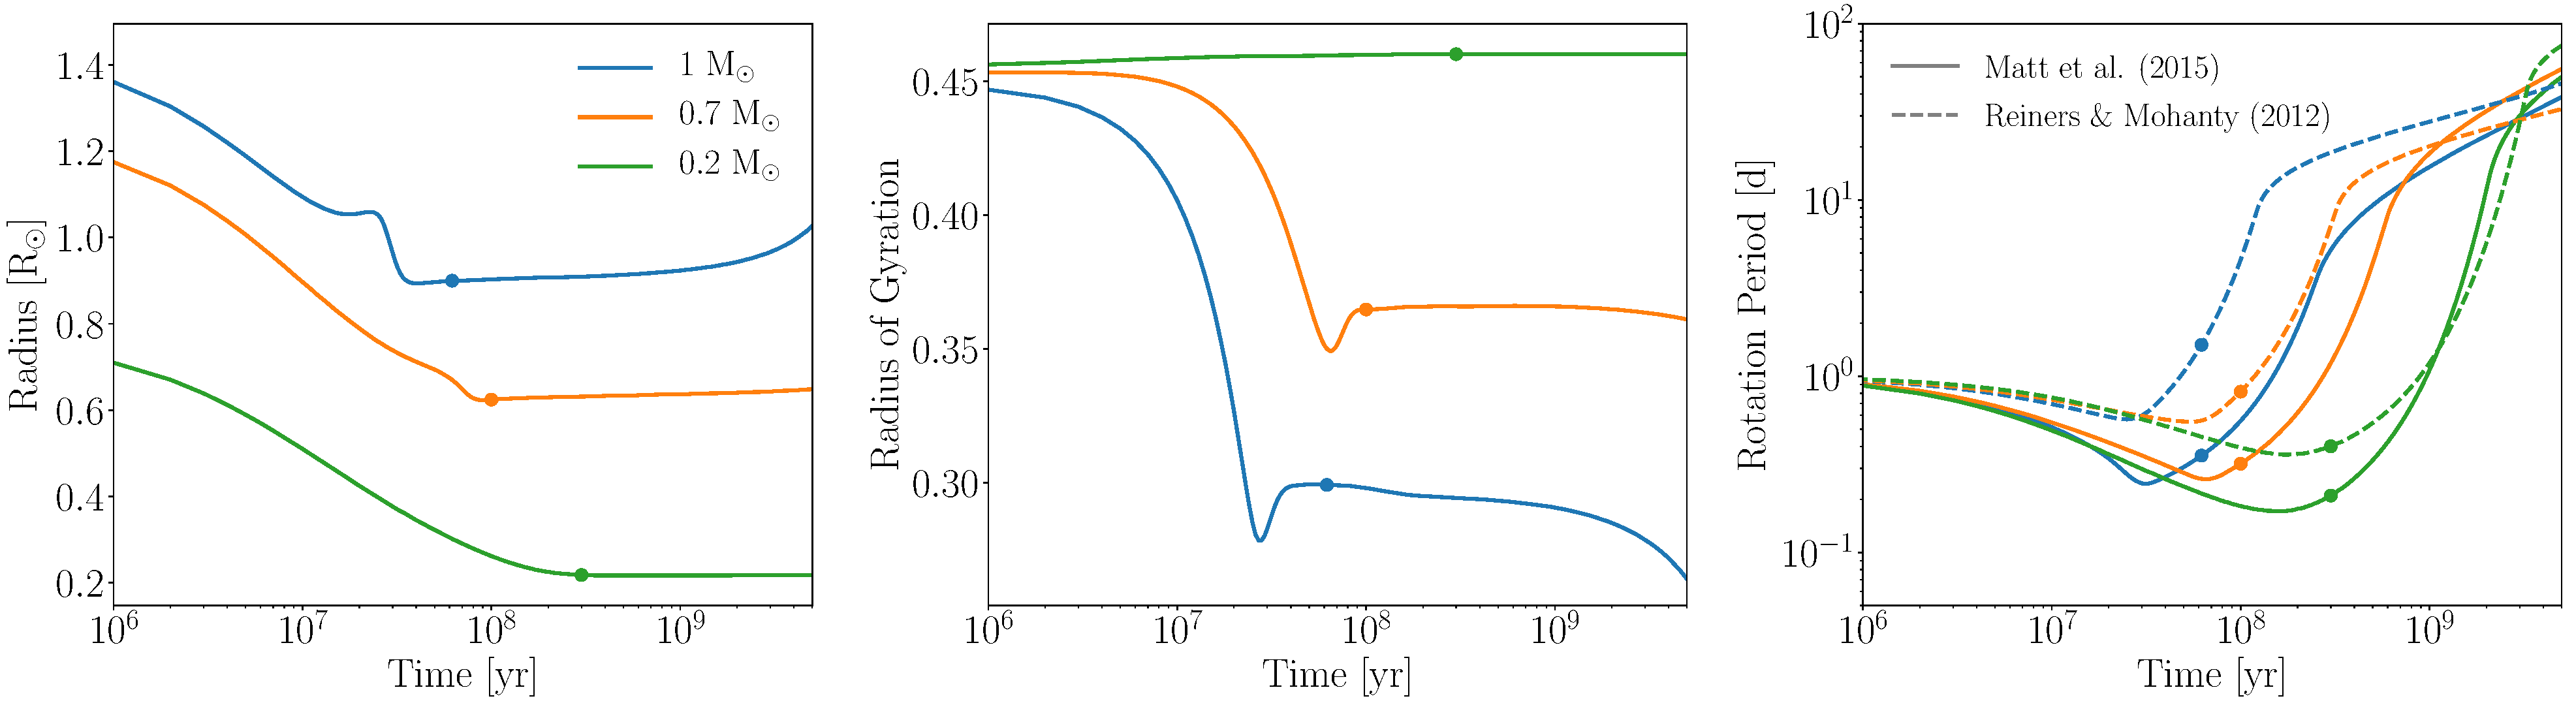
\includegraphics[width=\textwidth]{../Plots/stellarExample.pdf}
   \caption{Stellar radius (left), $r_g$ (middle), and P$_{rot}$ (right) evolution for 0.2 M$_{\odot}$ (M, green), 0.7 M$_{\odot}$ (K, orange), and 1 M$_{\odot}$ (G, blue) mass stars computed according to \stellar, our interpolation of the \citet{Baraffe2015} stellar evolution models ($\S$~\ref{sec:methods:stellar}) combined with the \citet{Matt2015} magnetic braking law. Each dot denotes the approximate time when each star reaches the main sequence.}%
    \label{fig:stellarExample}%
\end{figure*}

\subsection{Tidal Evolution} \label{sec:methods:eqtide}

 Equilibrium tidal models, first introduced by \citep{Darwin1880}, track the secular evolution of an orbiter's semi-major axis, $a$, eccentricity, $e$, and the rotation rates, $\omega$, and obliquities $\psi$, of the both gravitating bodies due to tidal torques. Equilibrium tidal models assume that tidally-interacting bodies raise tidal bulges on their companions that remain offset from the line connecting the both bodies' centers of mass due to friction within each body.  The tidal bulges cause torques that drive the exchange of angular momentum between the orbit and both bodies' spins. Equilibrium tidal models are linear since they assume that the tidal waves that comprise the tidal bulge raised on a body are uncoupled. Under these assumptions, the tidal evolution is analogous to a driven, damped harmonic oscillator \citep{Greenberg2009}.  We refer the reader to \citet{Barnes2017} for an in-depth discussion of the assumptions and limitations of equilibrium tidal models.  Although simple, equilibrium tidal models have been used to robustly model the secular orbital and rotation evolution of both Solar System bodies and exoplanets \citet[e.g.][]{Goldreich1966,Jackson2009,Leconte2010,Heller2011,Barnes2013,Barnes2017} and stellar binaries \citep[e.g.][]{Zahn1989,Zahn2008,Khaliullin2011,Repetto2014,Fleming2018}.  Here, we consider two equilibrium tidal models to study the secular spin-orbital evolution of low-mass stellar binaries.  

\subsubsection{Constant Phase Lag Model}

The ``Constant Phase Lag" (CPL) \citep[][]{FerrazMello2008,Heller2011} equilibrium tidal model assumes that the tidal torque on one body due to its companion arises from a linear combination of several discrete, uncoupled tidal bulges, each with their own associated frequency, that maintain a fixed phase with respect to the line connecting the two stars' centers of mass. We use the \eqtide implementation of the CPL model in VPLanet following the derivation of \citet{FerrazMello2008}.  The equations that govern the secular change in $e$ and $a$ are as follows:

\begin{equation} \label{eqn:cpl:e}
\frac{de}{dt} = -\frac{ae}{8 G m_1 m_2} \sum_{i=1}^2 Z_{i,\mathrm{CPL}} \left( 2 \varepsilon_{0,i} - \frac{49}{2} \varepsilon_{1,i} + \frac{1}{2} \varepsilon_{2,i} + 3 \varepsilon_{5,i} \right)
\end{equation}
\begin{equation} \label{eqn:cpl:a}
\frac{da}{dt} = \sum_{i=1}^2 \frac{da_i}{dt}
\end{equation}
where if the $i^{th}$ body is tidally-locked in a synchronous orbit,
\begin{equation} \label{eqn:cpl:dadt_locked}
\frac{da_{i,sync}}{dt} = -\frac{a^2}{G m_1 m_2} Z_{i,\mathrm{CPL}} \left( 7 e^2 + \sin^2 (\psi_i) \right) \varepsilon_{2,i},
\end{equation}
otherwise
\begin{equation}
\begin{split}
\frac{da_i}{dt} & = \frac{a^2}{4 G m_1 m_2} Z_{i,\mathrm{CPL}} \left( 4 \varepsilon_{0,i} + e^2 \left[ -20 \varepsilon_{0,i} + \frac{147}{2} \varepsilon_{1,i} \right. \right. \\
&  + \left. \left. \frac{1}{2} \varepsilon_{2,i} - 3 \varepsilon_{5,i} \right] - 4 \sin^2 (\psi_i) \left[ \varepsilon_{0,i} - \varepsilon_{8,i} \right] \right).
\end{split}
\end{equation}
The CPL equations for $\psi$ and $\omega$ evolution are
\begin{equation} \label{eqn:cpl:psi}
\frac{d\psi_i}{dt} = \frac{Z_{i,\mathrm{CPL}} \sin(\psi_i)}{4 m_i r_{g,i}^2 R_i^2 n \omega_i} \left( [1-\xi_i] \varepsilon_{0,i} + [1+\xi_i](\varepsilon_{8,i} - \varepsilon_{9,i}) \right)
\end{equation}
\begin{equation} \label{eqn:cpl:omega}
\begin{split}
\frac{d\omega_i}{dt}& = -\frac{Z_{i,\mathrm{CPL}}}{8m_i r_{g,i}^2 R_i^2 n} \left(4 \varepsilon_{0,i} + e^2\left[-20\varepsilon_{0,i} + 49\varepsilon_{1,i} + \varepsilon_{2,i} \right] \right. \\
& \left. + 2 \sin^2(\psi_i) \left[ -2 \varepsilon_{0,i} + \varepsilon_{8,i} + \varepsilon_{9,i} \right] \right)
\end{split}
\end{equation}
where $G$ is Newton's gravitational constant, $n$ is the binary's mean motion, and the index $i$ denotes that $i^{th}$ body. The tidal phase lags signs, $\varepsilon$, for the $i^{th}$ body are given by
\begin{equation} \label{eqn:cpl:eps}
\begin{split}
\varepsilon_{0,i} & = \Sigma(2 \omega_i - 2n) \\
\varepsilon_{1,i} & = \Sigma(2 \omega_i - 3n) \\
\varepsilon_{2,i} & = \Sigma(2 \omega_i - n) \\
\varepsilon_{5,i} & = \Sigma(n) \\
\varepsilon_{8,i} & = \Sigma(\omega_i - 2n) \\
\varepsilon_{9,i} & = \Sigma(\omega_i)
\end{split}
\end{equation}
where the function $\Sigma(x)$ returns $1$ for positive $x$, $-1$ for negative $x$, and $0$ otherwise.

The intermediate variable $Z_{\mathrm{CPL},i}$ is given by
\begin{equation} \label{eqn:cpl:z}
Z_{i,\mathrm{CPL}} = 3 G^2 k_{2,i} M_j^2 (M_i + M_j) \frac{R_i^5}{a^9} \frac{1}{n Q_i}
\end{equation}
where the $j^{th}$ body is the $i^{th}$ body's companion, $k_{2}$ is the body's Love number of degree 2, and $Q$ is the tidal quality factor (``tidal Q"). The tidal Q parameterizes the energy dissipation due to tidal evolution, with lower tidal Qs, i.e. larger phase differences between the tidal bulges, driving more rapid tidal evolution.

The other intermediate variable, $\xi_i$, is defined as
\begin{equation}\label{eqn:cpl:chi}
\xi_i = \frac{r_{\mathrm{g},i}^2 R_i^2 \omega_i a n }{ G M_j}.
\end{equation}

\subsubsection{Constant Time Lag Model}

The ``Constant Time Lag" (CTL) \citep[][]{Hut1981,Leconte2010} equilibrium tidal model assumes a constant time interval between the body's tidal bulge and the passage of the tidally-interacting companion. In this formalism, unlike the CPL model, the CTL model is continuous over a range of tidal wave frequencies.  However if the assumption of linearity is relaxed, i.e. frequencies associate with tidal bulges are allowed to depend on a spin or orbital forcing frequency, then this model is only valid over a small range of frequencies \citep{Greenberg2009}, hence we do not make this assumption and hold the tidal time lag fixed. We use the \eqtide implementation of the CTL model in VPLanet following the derivation of \citet{Leconte2010}.  The equations that govern the secular changes in $e$, $a$, $\omega$, and $\psi$ are as follows:

\begin{equation} \label{eqn:ctl:e}
  \frac{de}{dt} = \frac{11 ae}{2 G M_1 M_2}
  \sum_{i = 1}^2 Z_{\mathrm{CTL},i} \left( \cos(\psi_i) \frac{f_4(e)}{\beta^{10}(e)}  \frac{\omega_i}{n} -\frac{18}{11} \frac{f_3(e)}{\beta^{13}(e)}\right),
\end{equation}

\begin{equation}\label{eqn:ctl:a}
  \frac{da}{dt} \ = \  \frac{2 a^2}{G M_1 M_2}
  \sum\limits_{i = 1}^2 Z_{\mathrm{CTL},i} \left( \cos(\psi_i) \frac{f_2(e)}{\beta^{12}(e)} \frac{\omega_i}{n} - \frac{f_1(e)}{\beta^{15}(e)}\right),
\end{equation}

\begin{equation}\label{eqn:ctl:omega}
  \frac{d\omega_i}{dt} \ = \ \frac{Z_{\mathrm{CTL},i}}{2 M_i r_{g,i}^2 
R_i^2 n} \left( 2 \cos(\psi_i) \frac{f_2(e)}{\beta^{12}(e)} - \left[ 1+\cos^2(\psi)
 \right] \frac{f_5(e)}{\beta^9(e)} 
\frac{\omega_i}{n} \right),  
\end{equation}
and
\begin{equation}\label{eqn:ctl:psi}
  \frac{d\psi_i}{dt} = \frac{Z_{\mathrm{CTL},i} \sin(\psi_i)}{2 M_i r_{g,i}^2 R_i^2 n \omega_i}\left( \left[ \cos(\psi_i) - \frac{\xi_i}{ \beta} \right] \frac{f_5(e)}{\beta^9(e)} \frac{\omega_i}{n} - 2 \frac{f_2(e)}{\beta^{12}(e)} \right).
\end{equation}
where the intermediate variables are given by 
\begin{equation}\label{eqn:ctl:z}
 Z_{i,\mathrm{CTL}} = 3 G^2 k_{2,i} M_j^2 (M_i+M_j) \frac{R_i^5}{a^9} \tau_i ,
\end{equation}
and 
\begin{equation}\label{eqn:ctl:f_e}
\begin{array}{l}
\beta(e) = \sqrt{1-e^2},\\
f_1(e) = 1 + \frac{31}{2} e^2 + \frac{255}{8} e^4 + \frac{185}{16} e^6 + \frac{25}{
64} e^8,\\
f_2(e) = 1 + \frac{15}{2} e^2 + \frac{45}{8} e^4 + \frac{5}{16} e^6,\\
f_3(e) = 1 + \frac{15}{4} e^2 + \frac{15}{8} e^4 + \frac{5}{64} e^6,\\
f_4(e) = 1 + \frac{3}{2} e^2 + \frac{1}{8} e^4,\\
f_5(e) = 1 + 3 e^2 + \frac{3}{8} e^4.
\end{array}
\end{equation}

In both the CPL and CTL model, We assume $k_2 = 0.5$. This choice of $k_2$ does not impact our results as $k_2$ is degenerate with Q in the CPL model, e.g. the $k_2/Q$ scaling in Eq.~(\ref{eqn:cpl:z}), and with $\tau$ in the CTL model, e.g. $k_2 \tau$ scaling in Eq.~(\ref{eqn:ctl:z}), so we instead examine how our results scale with $Q$ and $\tau$.  Any constraints we derive for $Q$ and $\tau$ can trivially be scaled to other values of $k_2$.

\subsubsection{Tidal Locking}

Tidal torques always drive a body towards the tidally-locked state. When a body tidally locks, tidal torques fix P$_{rot}$ to the equilibrium P$_{rot}$, P$_{eq}$.  Typically, tidal locking is understood in the context of a synchronized rotator, e.g. when P$_{rot} = $ P$_{eq} = $ P$_{orb}$. Although spin-orbit synchronization is an expected outcome of tidal evolution \citep{Counselman1973}, in general for tidally-locked bodies on non-circular orbits, both the CPL and CTL model predict pseudosynchronous, or supersynchronous rotation, e.g. Mercury's 3:2 spin-orbit resonance \citep[P$_{rot} = 2/3$ P$_{orb}$,][]{GoldreichPeale1966}.   

The CPL model, owing to its assumption of a finite number of discrete tidal lags, only permits a 1:1 and 3:2 spin-orbit state where, following \citet{Barnes2017}, the CPL P$_{eq}$ is given by
\begin{equation} \label{eqn:cpl:eqPer}
P^{\mathrm{CPL}}_{eq} = 
\begin{cases}
P_{orb} & \text{if } e < \sqrt{1/19}\\
\frac{2}{3}P_{orb} & \text{if } e \geq \sqrt{1/19}.
\end{cases}
\end{equation}
Therefore, the CPL model predicts synchronous rotation for $e \lsim 0.23$, and a supersychronous 3:2 spin-orbit state otherwise.

The CTL model, however, is continuous over a range of tidal frequencies and therefore predicts a P$_{eq}$ that is a continuous function of both $e$ and $\psi$.  Following \citet{Barnes2017}, we define the CTL P$_{eq}$ by
\begin{equation} \label{eqn:ctl:eqPer}
P^{\mathrm{CTL}}_{eq} = P_{orb} \frac{\beta^3 f_5(e) (1 + \cos^2(\psi))}{2f_2(e) \cos(\psi)}.
\end{equation}
The CTL model predicts that bodies on eccentric orbits tidally-lock into supersyncronous rotation, and only bodies with aligned spins on circular orbits are synchronous rotators. 

Due to the discontinuities in the equilibrium tidal model equations, for example in Eq.~(\ref{eqn:cpl:eps}) when $\omega \approx n$, and due to the inherant discreteness of numerical integrations, numerical solutions for the CPL and CTL models can produce unphysical evolution. We follow \citet{Barnes2013} and \citet{Fleming2018} and fix P$_{rot} = $ P$_{eq}$ according to Eq.~(\ref{eqn:cpl:eqPer}) or Eq.~(\ref{eqn:ctl:eqPer}) for the CPL and CTL models, respectively when P$_{rot}$ is within $1\%$ of P$_{eq}$.  To ensure that tidal torques dominate over torques due to magnetic braking and stellar evolution, we additionally require that the P$_{rot}$ derivative points towards $P_{eq}$ on both sides of P$_{eq}$, i.e. when the gradient of P$_{rot}$ points towards the tidally-locked state, before fixing P$_{rot} = $ P$_{eq}$. We find that this scheme produces physically and numerically accurate results. 

\subsubsection{Example Tidal Evolution} \label{sec:methods:eqtideExample}

We plot the tidal evolution for $a$, $e$, and $\omega$, ignoring stellar evolution, for a solar-twin binary with an initial P$_{orb} = 10$ d, P$_{rot} = 1$ d, $e = 0.2$ for the CPL model and CTL model, assuming $Q=10^6$ and $\tau = 0.1$ seconds, respectively, in Fig.~\ref{fig:tidalExample}. Both the CPL and CTL model predict the same qualitative evolution: both the binary's $e$ and P$_{orb}$ slightly increasing as tides force the spins toward the tidally-locked state, transfering rotational angular momentum into the orbit in the process.  At late times, both the CPL and CTL drive the binaries towards orbital circularization, with tidal dissipation decreasing P$_{orb}$. The predictions of the CPL and CTL model, differ, however, when the binaries tidally-lock.  Under the CPL model, the binary tidally-locks into a synchronous orbit as $e < \sqrt{1/19}$, e.g. Eq.~(\ref{eqn:cpl:eqPer}), while the CTL model predicts supersyncronous rotation due to the CTL model's equilibrium period eccentricity dependence, e.g. Eq.~(\ref{eqn:ctl:eqPer}).

\begin{figure}
	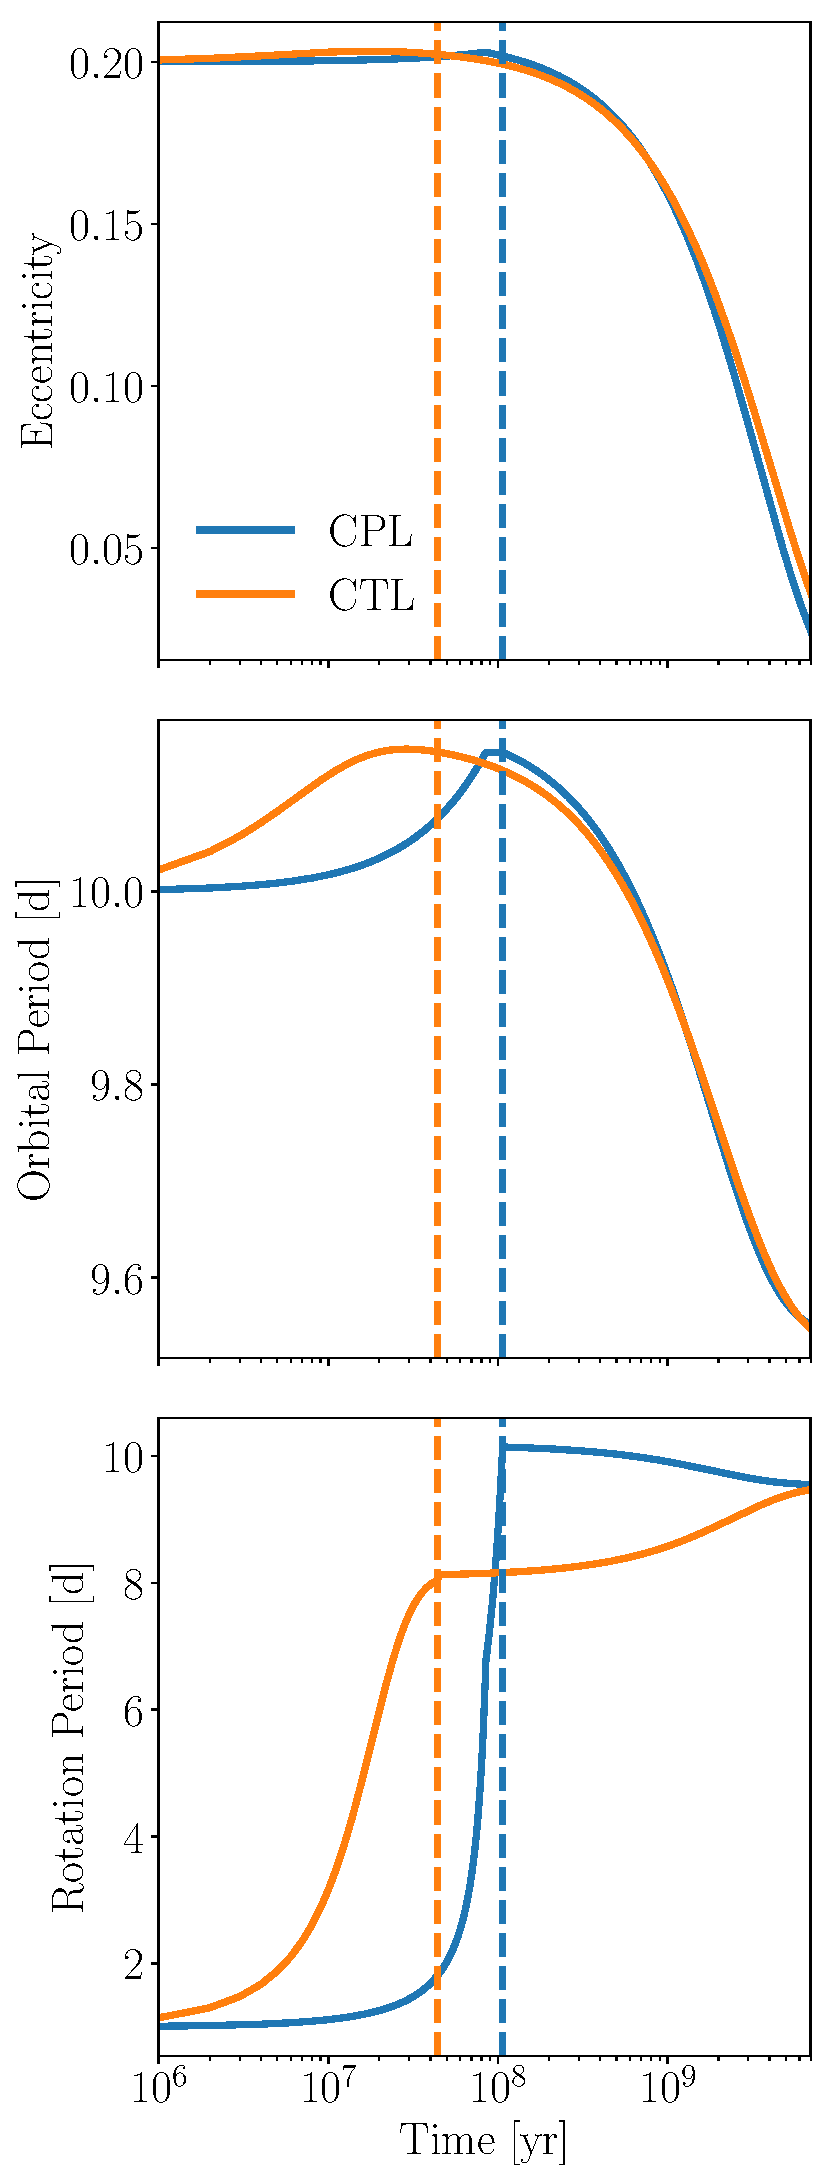
\includegraphics[width=0.4\textwidth]{../Plots/tidalExample.pdf}
   \caption{Tidal evolution of a 1 M$_{\odot} -$ 1 M$_{\odot}$ stellar binary's $e$ (top), P$_{orb}$ (middle) and P$_{rot}$ (bottom) for the CPL (blue) and CTL (orange) model. The blue (CPL) and orange (CTL) vertical dashed lines denote when the stellar binary tidally-locks. Both the CPL and CTL model predict the same qualitative evolution. The rotational evolution differs, however, as under the CPL model, the binary tidally-locks into a synchronous orbit as $e < \sqrt{1/19}$, e.g. Eq.~(\ref{eqn:cpl:eqPer}), while the CTL model predicts supersyncronous rotation due to the CTL model's equilibrium period eccentricity dependence (see Eq.~(\ref{eqn:ctl:eqPer})).}%
    \label{fig:tidalExample}%
\end{figure}

\subsection{Coupled Stellar-Tidal Evolution} \label{sec:coupled}

Following \citet{Fleming2018}, when one or both binary stars are tidally locked, we assume that tidal forces prevent magnetic braking from spinning down the tidally-locked star(s), but instead, any angular momentum lost is lost at the expense of the binary orbit, decreasing $a$ as a result \citep{Verbunt1981}.  Below in Eq.~(\ref{eqn:tidal_locked_one}) and Eq.~(\ref{eqn:tidal_locked_two}), we modify the $a$ decay equations due to stellar evolution and magnetic braking in tidally-locked binaries from \citet{Fleming2018}, their Eqs. (18) and (20), to additionally account for $r_g$ evolution when one or both stars tidally-lock, respectively, assuming conservation of angular momentum:
\small
\begin{equation} \label{eqn:tidal_locked_one}
\begin{split}
\dot{a}_{coupled}^{(1)} = \frac{-\dot{J}_{mb} - 2 \omega \left( m_1 r_{g,1}^2 R_1 \dot{R_1} - m_1 r_{g,1} \dot{r}_{g,1} R_1^2 \right)}
{\frac{\mu^2 G M (1-e^2)}{2J_{orb}} - \frac{3 \omega}{2a} m_1 r_{g,1}^2 R_1^2}
\end{split}
\end{equation}
\normalsize
and
\small
\begin{equation} \label{eqn:tidal_locked_two}
\begin{split}
\dot{a}_{coupled}^{(2)} = \frac{-\dot{J}_{mb} - 2 \omega \left( \sum_{i=1}^{2} m_i r_{g,i}^2 R_i \dot{R_i} + m_i r_{g,i} \dot{r}_{g,i} R_i^2 \right)}
{\frac{\mu^2 G M (1-e^2)}{2J_{orb}} - \frac{3 \omega}{2a} \left( m_1 r_{g,1}^2 R_1^2 + m_2 r_{g,2}^2 R_2^2 \right)}.
\end{split}
\end{equation}
\normalsize
where $J_{orb}$ is the orbital angular momentum.

%% SECTION: Simulations + Initial conditions %%
\section{Simulations} \label{sec:simulations}

We examine stellar angular momentum evolution in low-mass binaries by performing a Monte Carlo study of two sets of 10,000 stellar binaries, one modeled using the CPL model and the other using the CTL formalism.  We simulate both stars' spin evolution but mainly consider the P$_{rot}$ evolution for the primary, i.e. more massive star in binaries, as it is observationally easier to measure a P$_{rot}$ on the more massive, and hence brighter, star \citep[e.g.][]{Meibom2006,Lurie2017}. For each simulation, we sample the primary's mass uniformly over $[0.1, 1]$ M$_{\odot}$. Following \citet{Matt2015}, we uniformly sample the log$_{10}$ of P$_{rot}$ over [$0.8,15$] days, a distribution that approximates the P$_{rot}$ distribution of young stars in the ${\sim}2$ Myr old ONC.  We compute the secondary star's mass by uniformly sampling the mass ratio over [$0.1, 1$] following observations of mass ratios in low-mass binaries \citep{Raghavan2010,Moe2018}. Given the inherent uncertainty in and complexity of the formation of binaries \citep[e.g.][]{Bonnell1994,Bate2000,Bate2002,Moe2018} and the potential for dynamical processing via tides or stellar close encounters \citep[e.g.][]{Mardling2001,Hurley2002,Ivanova2005,Meibom2005}, we take an agnostic approach to the initial orbital configuration by uniformly randomly sampling the initial eccentricity ($e$) over [$0.0,0.3$] and uniformly sampling the initial P$_{orb}$ over [$3,100$] d. Altough the CTL model is applicable for $e > 0.3$ while the CPL model is not, we restrict $e \leq 0.3$ to allow us to compare both models.

Values for stellar tidal $Q$s and $\tau$s for low-mass stars are highly uncertain, likely depend on complex viscous evolution within the stars \citep{Ogilvie2007}, differ for stars of the same spectral clase \citep{Barker2009}, and can vary as a function of stellar age \citep{Bolmont2016}. Typical values of $Q$ and $\tau$ for Sun-like stars are estimated to be of order $Q \approx 10^6$ and $\tau \approx 0.1$ s, respectfully \citep[e.g.][]{Meibom2005,Ogilvie2007,Jackson2009}, however a wide range of values exist in the literature.  Therefore, we consider a wide range of tidal parameters and sample stellar tidal Qs loguniformly over $[10^4,10^7]$ and $\tau$ loguniformly over $[10^{-2},1]$ s.

All code used to run simulations and generate figures is available online\footnote{\href{https://github.com/dflemin3/sync}{https://github.com/dflemin3/sync}.} with accompanying descriptions and documentation.

%% SECTION: RESULTS %%

\section{Role $Q$ and $\tau$}

we can explain fast rotation observed in \citet{Meibom2007} to be due to tidal torques speeding up stellar Prots

\begin{figure}
	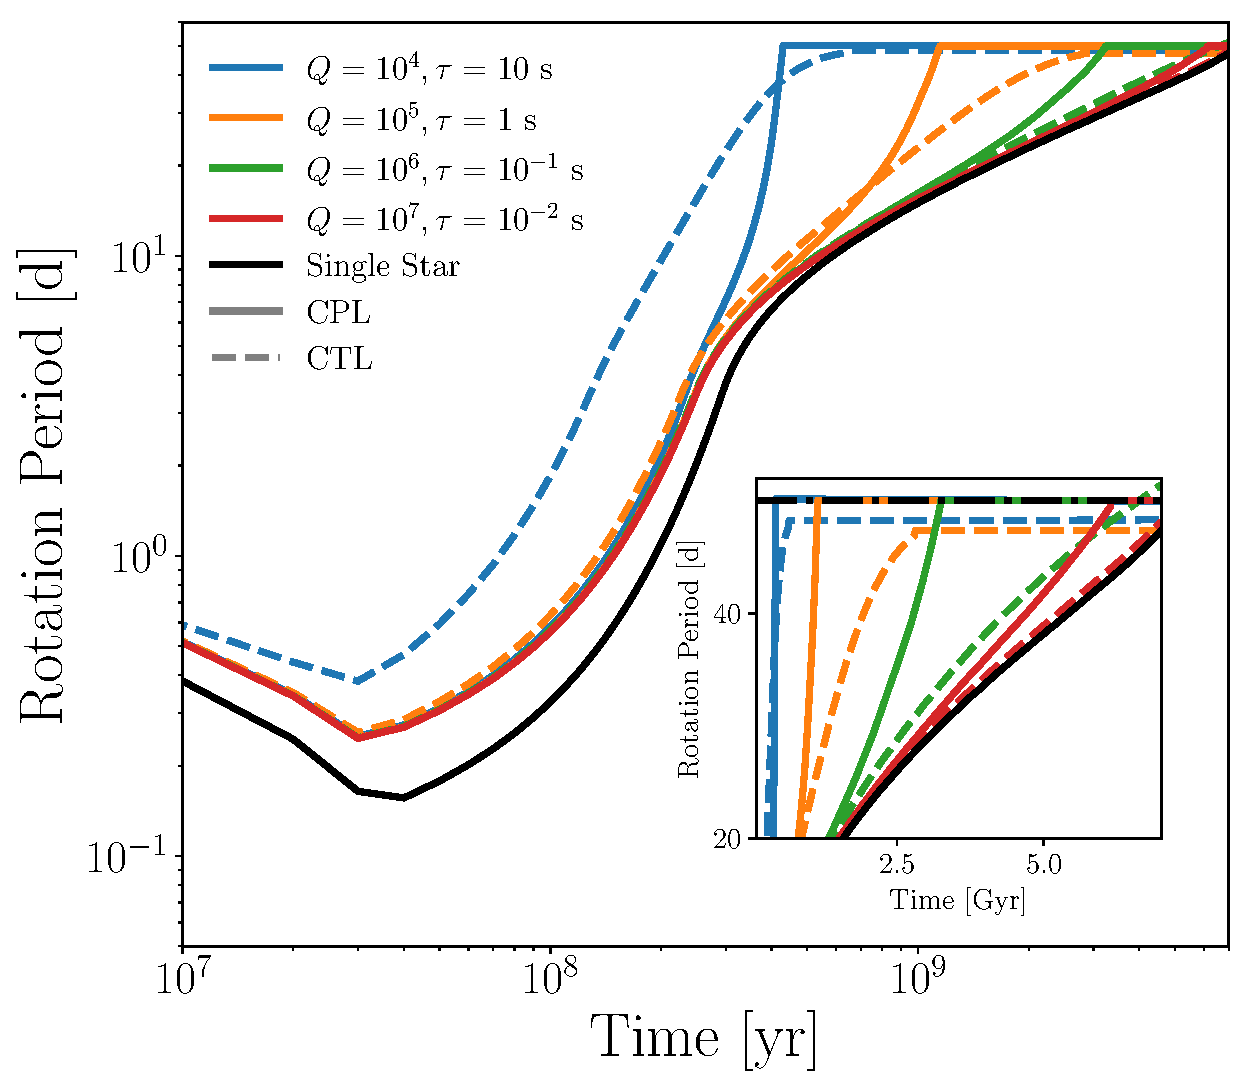
\includegraphics[width=0.45\textwidth]{../Plots/example.pdf}
   \caption{Caption.}%
    \label{fig:coupledExample}%
\end{figure}

XXX

\begin{figure}
	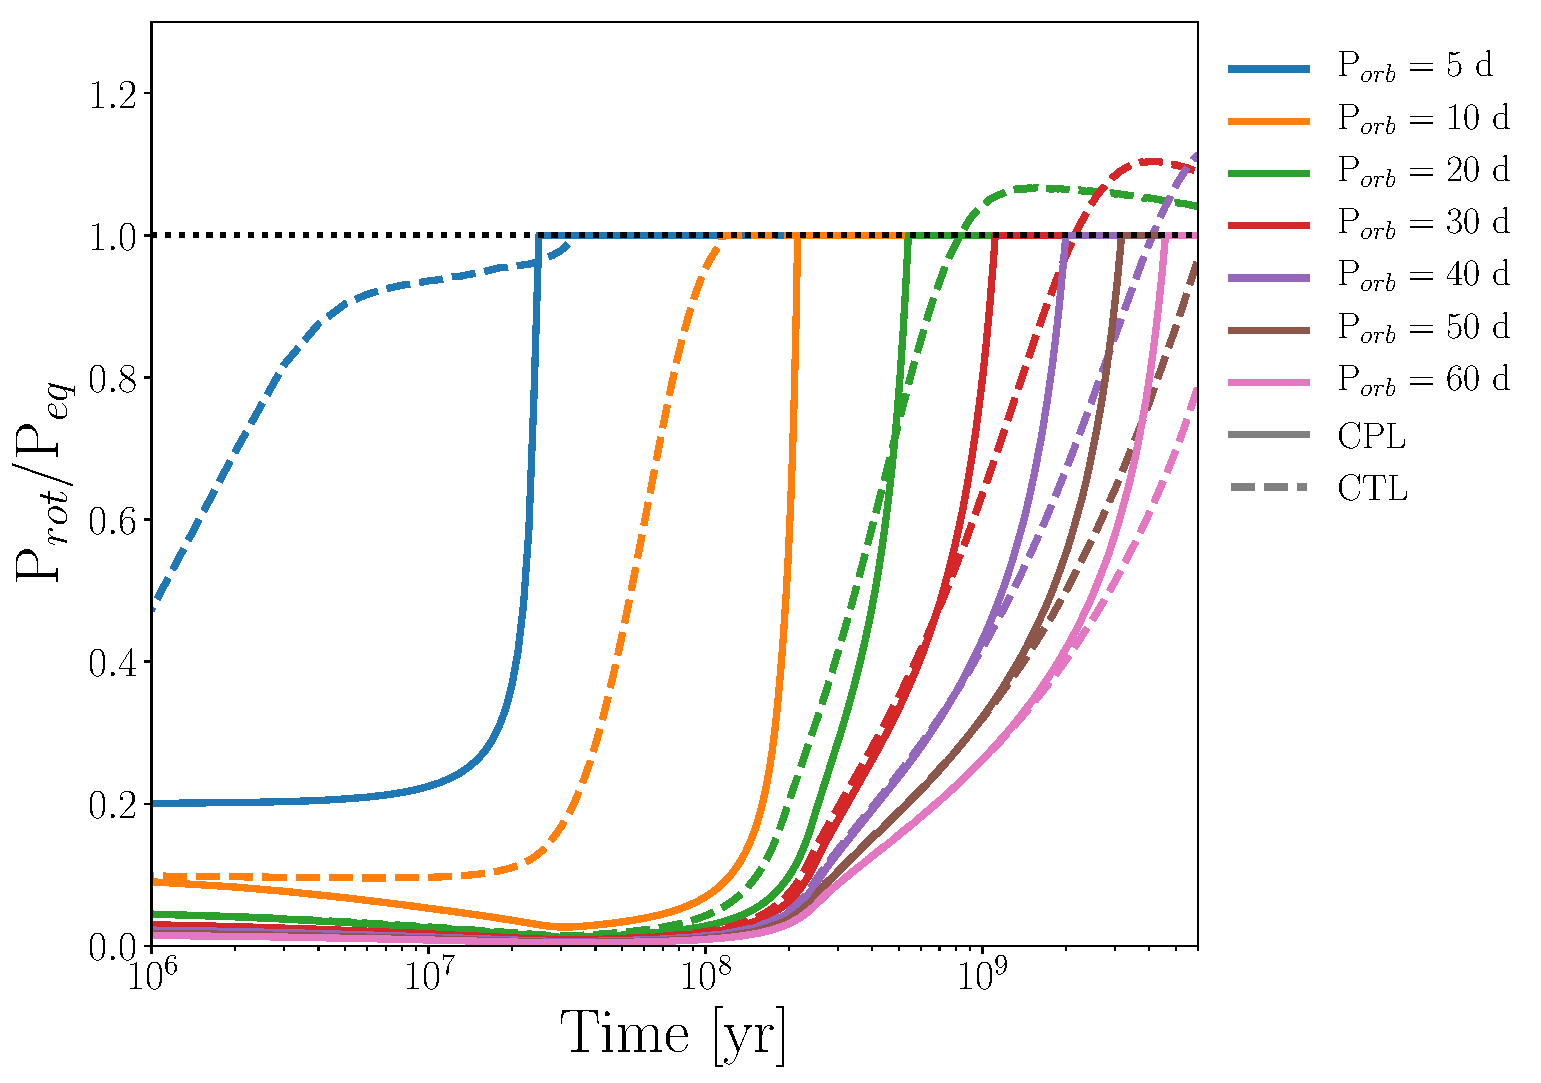
\includegraphics[width=0.45\textwidth]{../Plots/eqPer.pdf}
   \caption{Caption.}%
    \label{fig:eqPer}%
\end{figure}

XXX

\begin{figure*}[ht]
	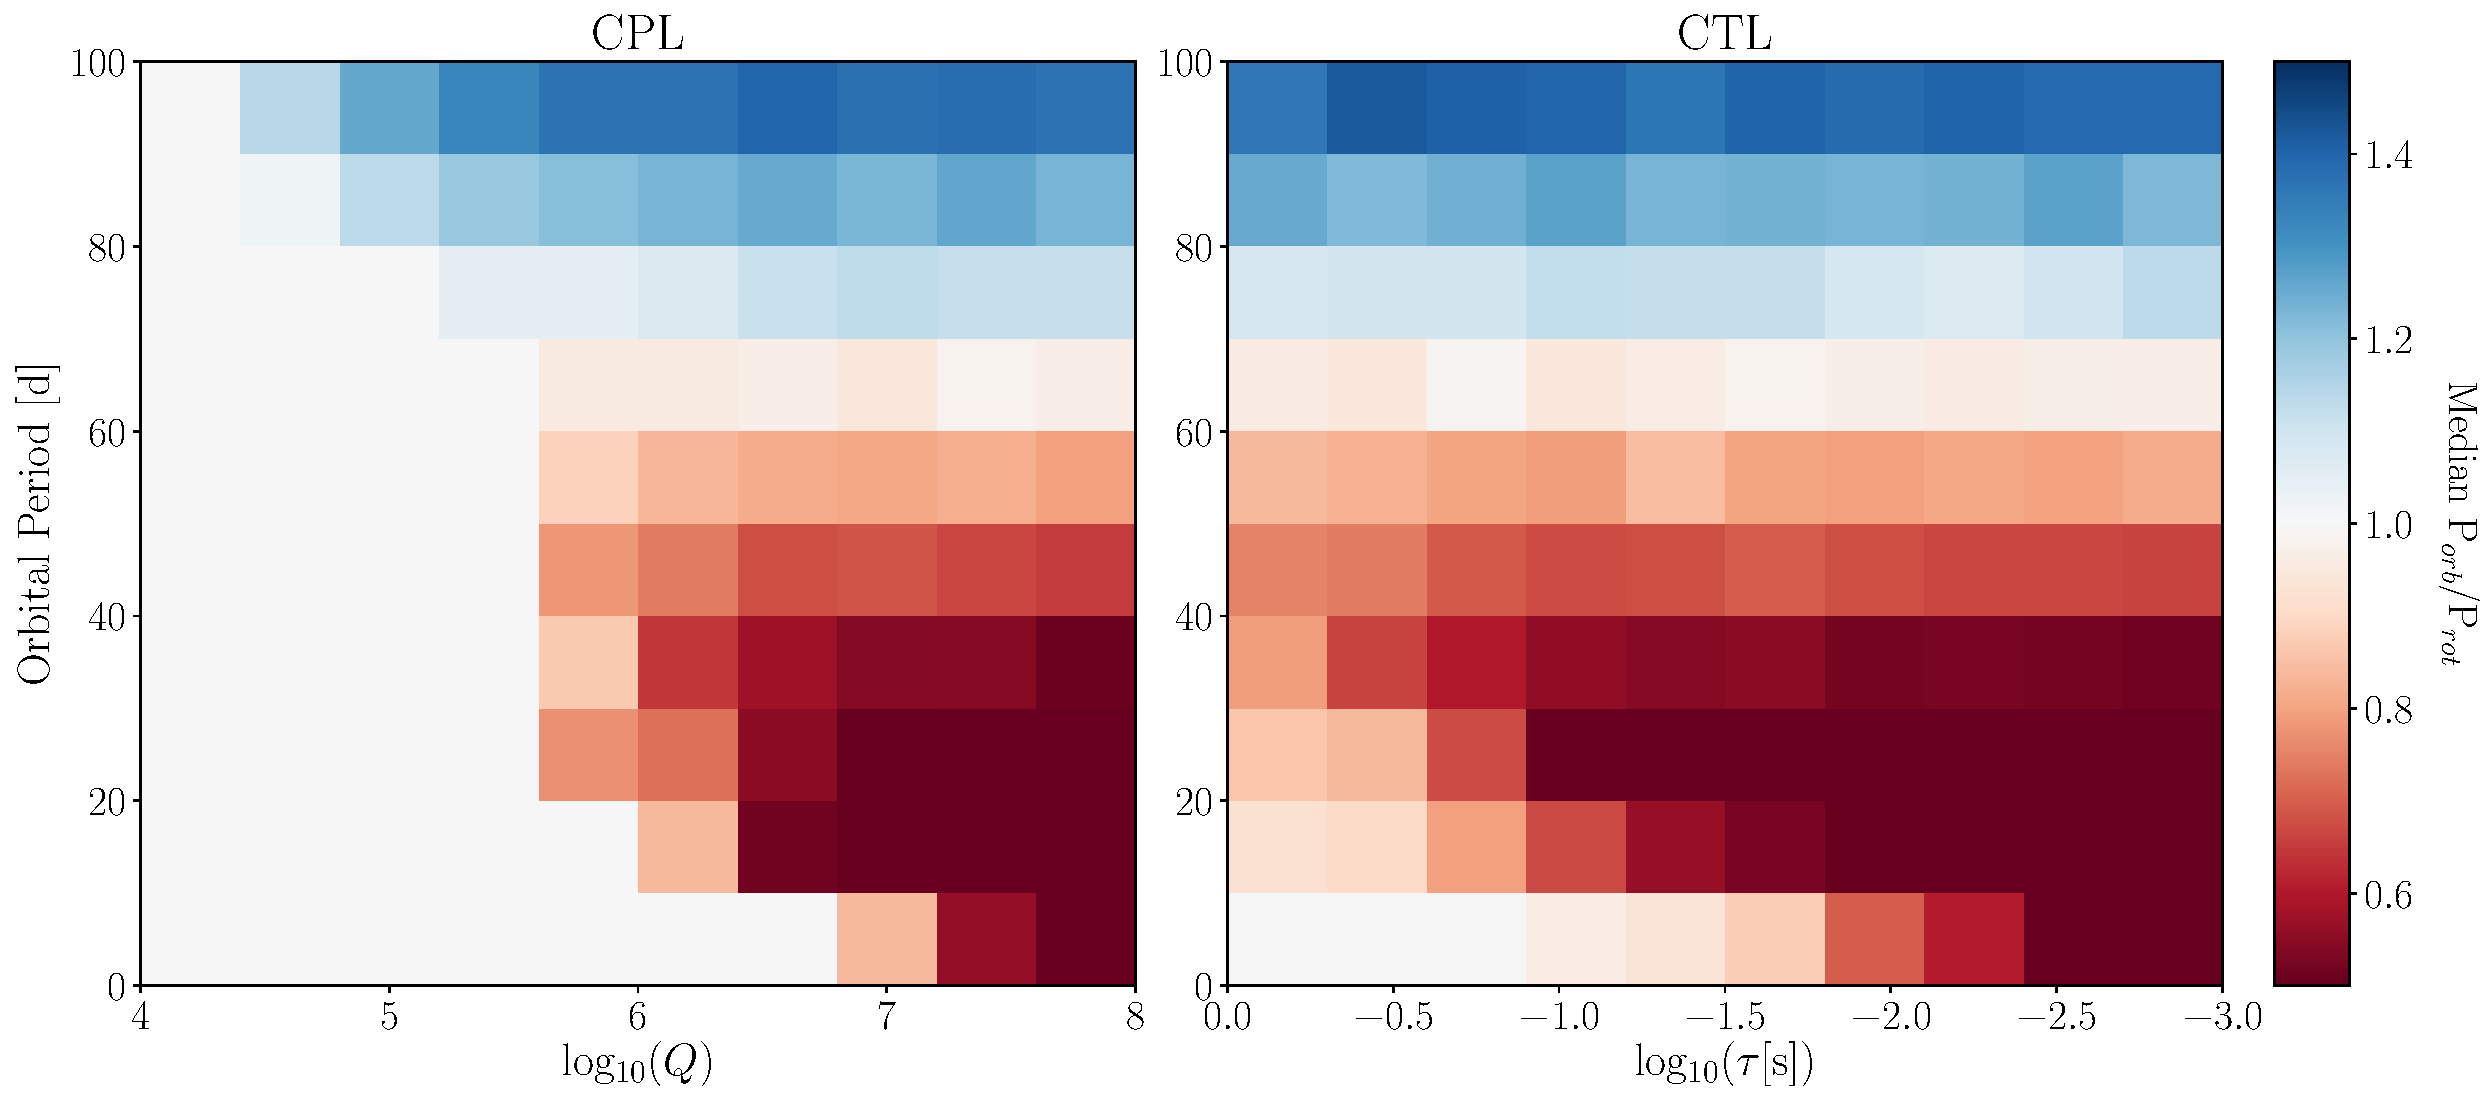
\includegraphics[width=\textwidth]{../Plots/qTauPorbRatioHist.pdf}
   \caption{Caption}%
    \label{fig:qTauLock}%
\end{figure*}

XXX

\begin{figure}
	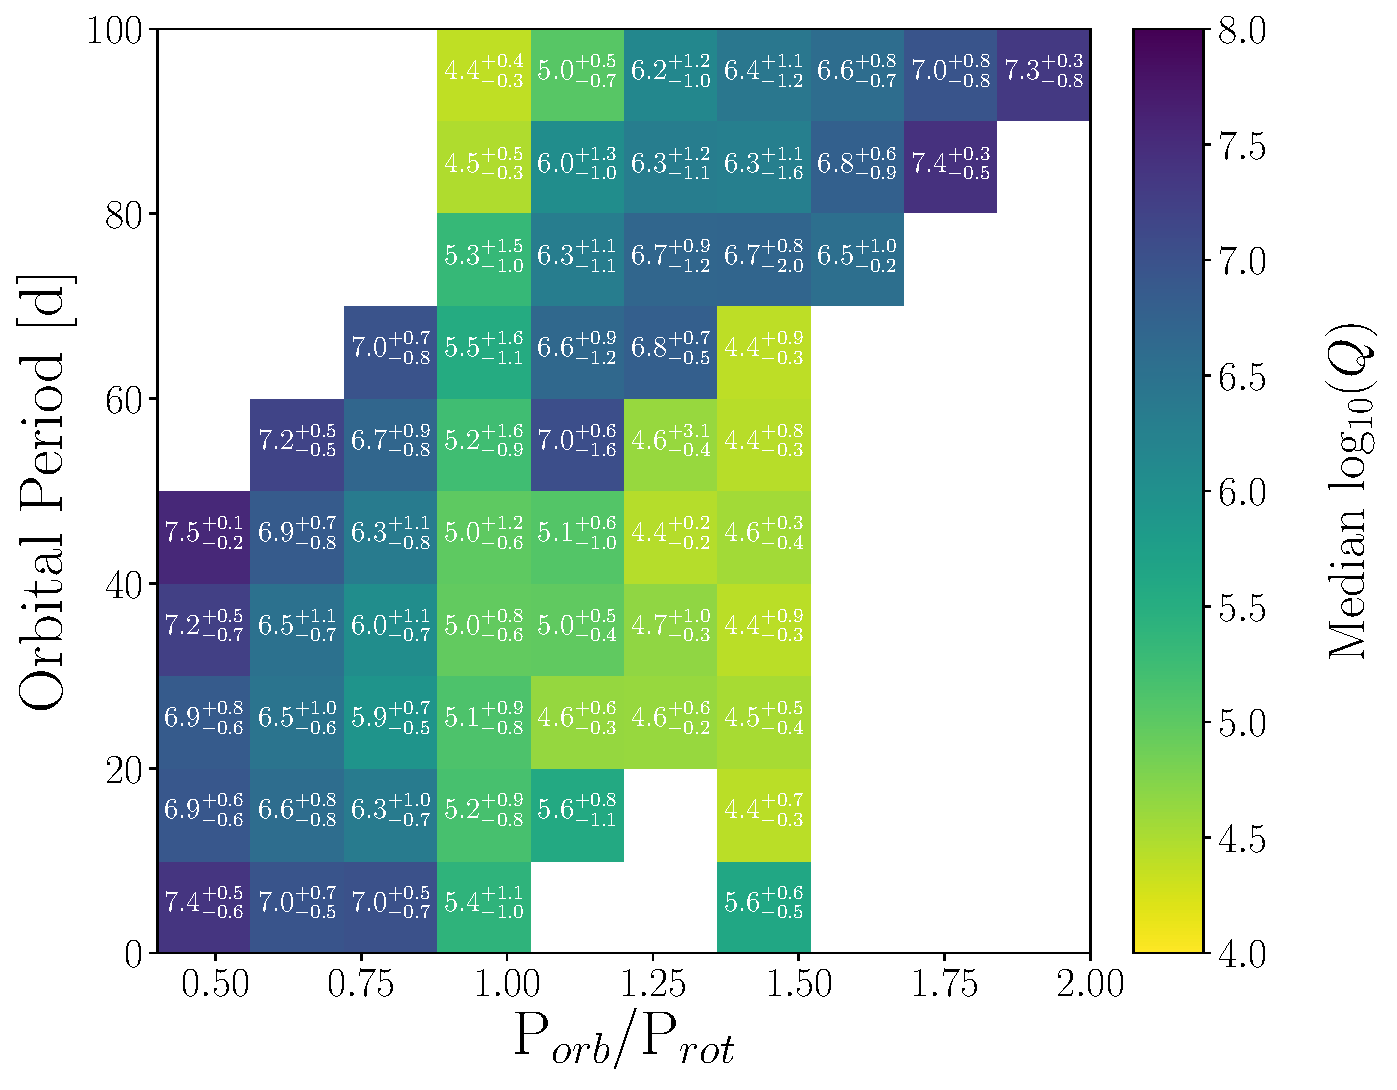
\includegraphics[width=0.45\textwidth]{../Plots/porbProtPorbQHist.pdf}
   \caption{Caption}%
    \label{fig:qmap}%
\end{figure}

XXX

\begin{figure}
	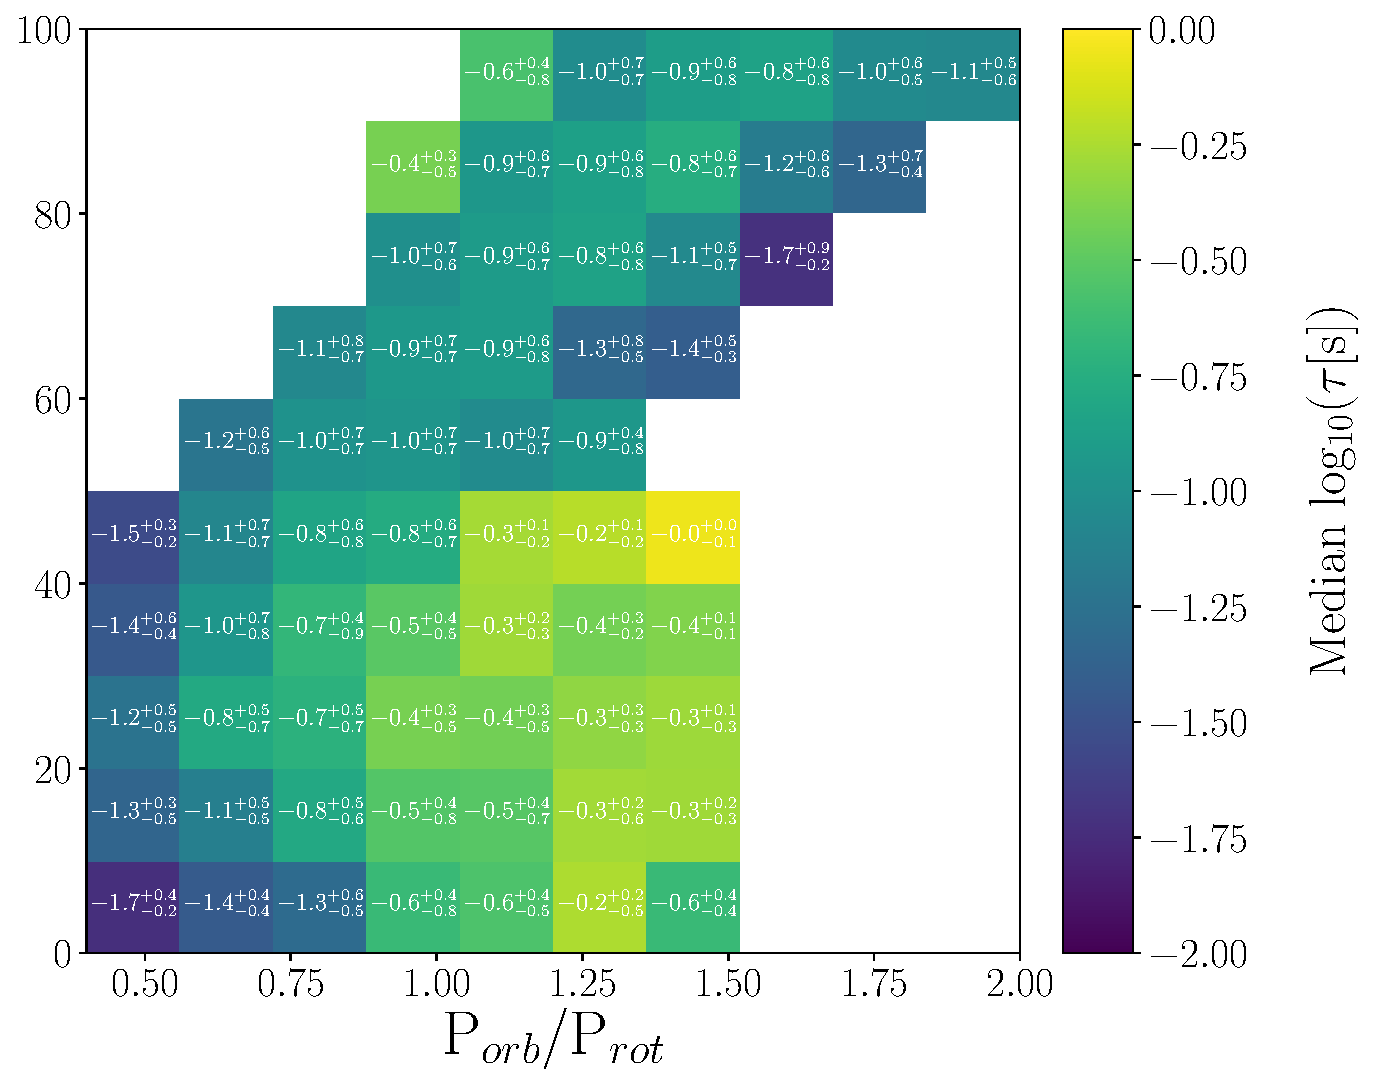
\includegraphics[width=0.45\textwidth]{../Plots/porbProtPorbTauHist.pdf}
   \caption{Caption}%
    \label{fig:taumap}%
\end{figure}

XXX

\section{Deviations From Single Star P$_{rot}$ Evolution: Implications for Gyrochronology} \label{sec:gyro}

\begin{figure}
	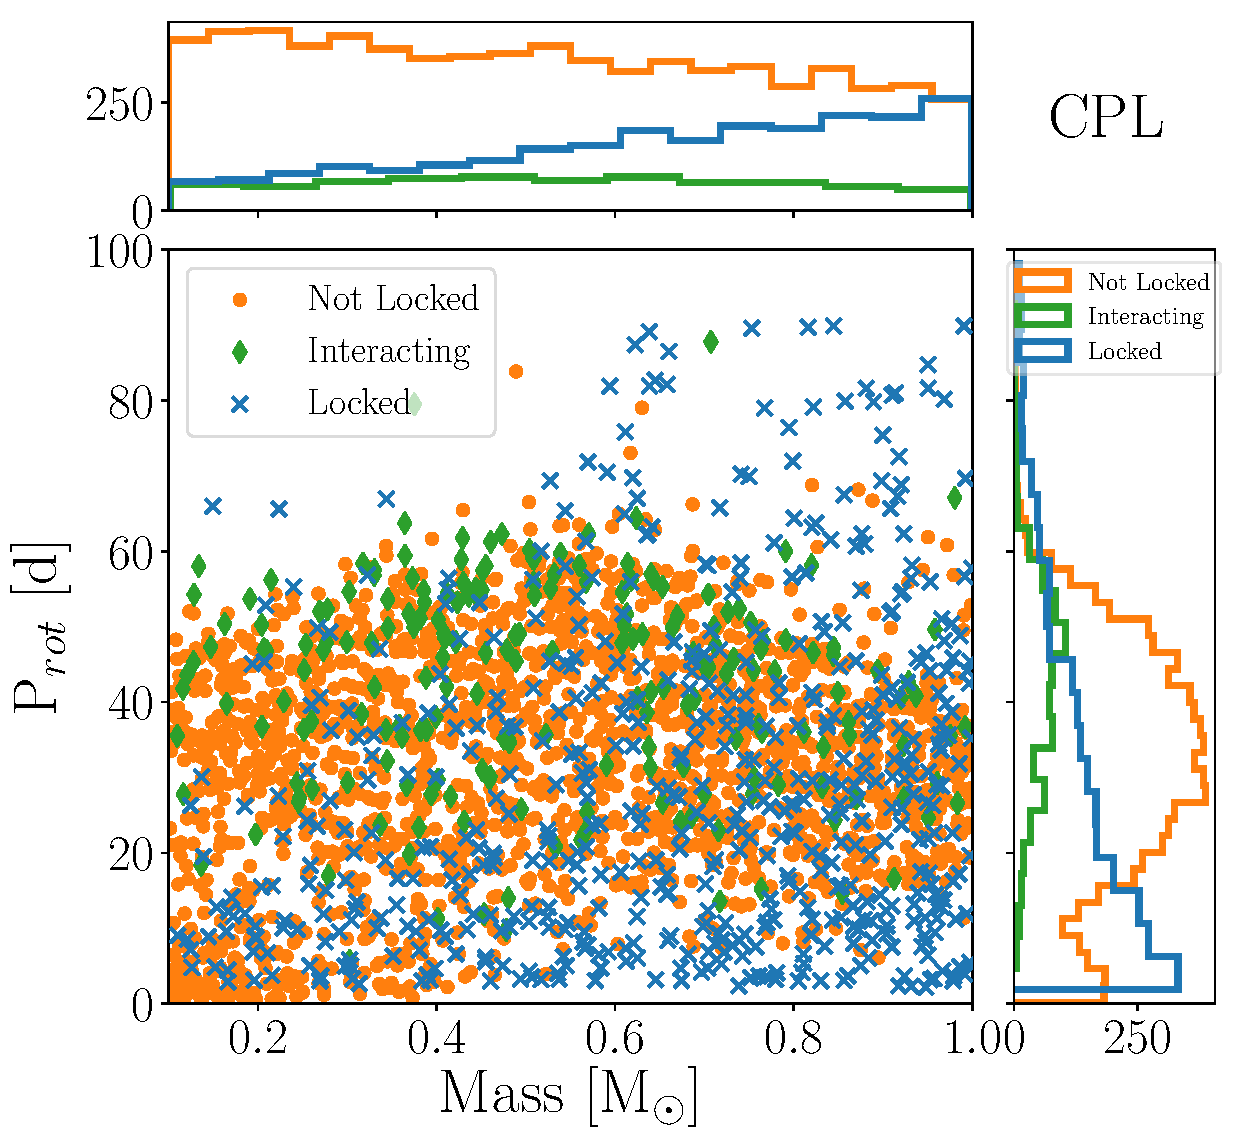
\includegraphics[width=0.45\textwidth]{../Plots/lockedCPL.pdf}
   \caption{Caption.}%
    \label{fig:lockedCPL}%
\end{figure}

XXX

\begin{figure}
	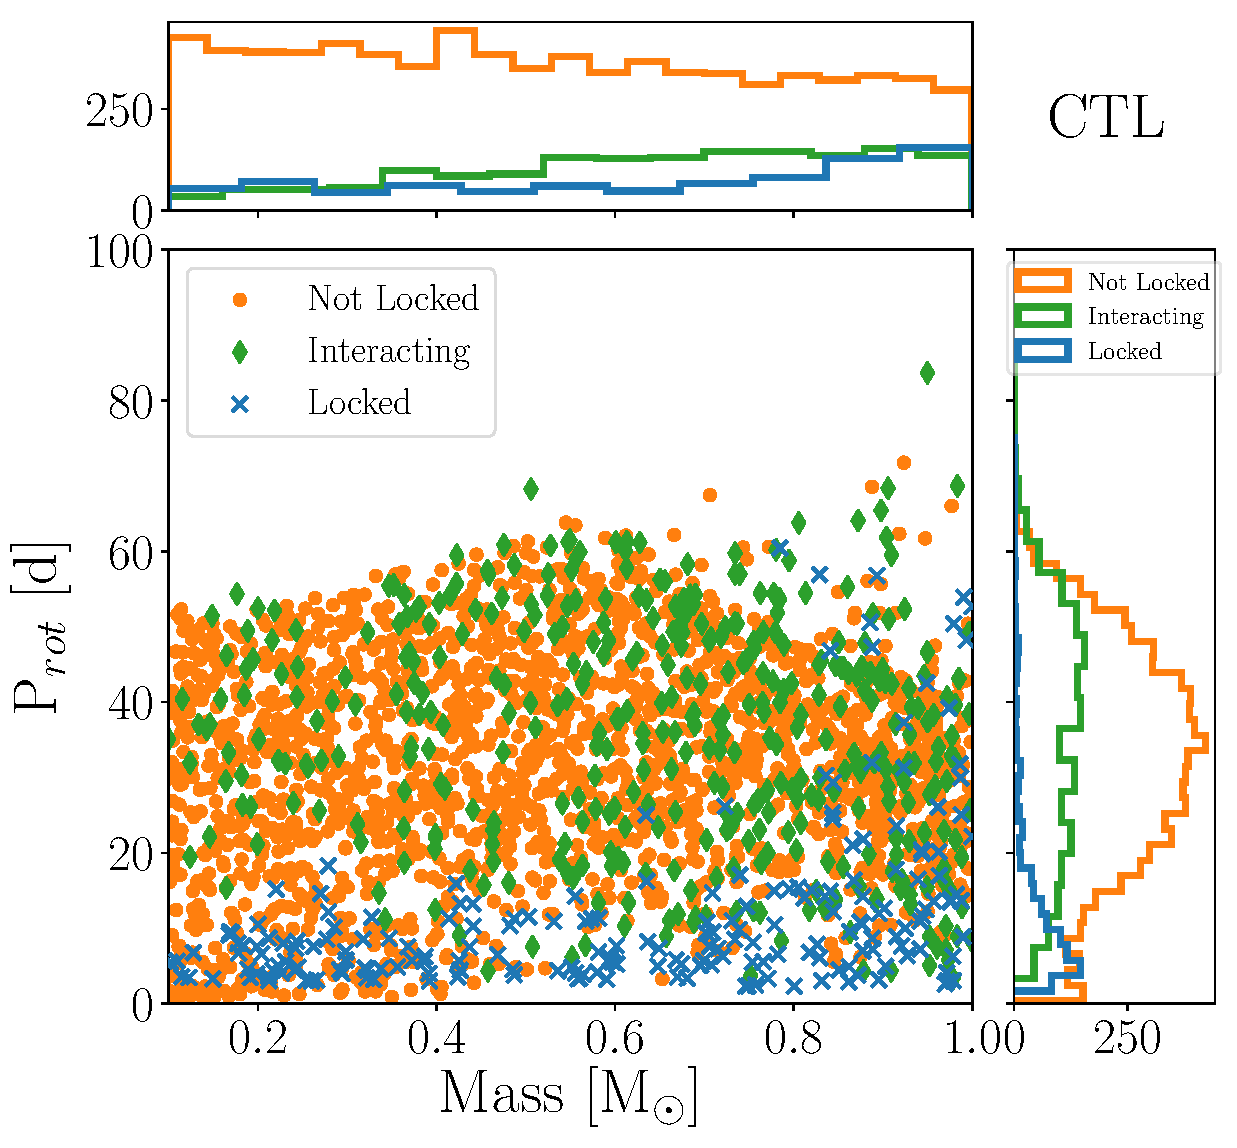
\includegraphics[width=0.45\textwidth]{../Plots/lockedCTL.pdf}
   \caption{Caption.}%
    \label{fig:lockedCTL}%
\end{figure}

XXX

Here we compare the P$_{rot}$ distribution for tidally-interacting stellar binaries from our CPL and CTL simulations with the P$_{rot}$ distribution of single stars subject to stellar evolution and magnetic braking.  We simulate 10,000 single star systems according to the evolution described in $\S$~\ref{sec:methods:stellar}.  To generate the simulations, we sample from the same mass and initial P$_{rot}$ distributions we used for the binary simulations described $\S$~\ref{sec:methods}. In Fig.~\ref{fig:protDist}, we P$_{rot}$ as a function of mass and age for binaries simulated using both the CPL and CTL model and for single stars. 

Tidally-locked binaries tend to rotate more rapidly than unlocked binaries, reflected in the increased density for P$_{rot} \lsim 20$ d in the marginal distribution for the locked population and in the distribution medians (locked median P$_{rot} = 19.8$ d compared to unlocked median P$_{rot} = 27.5$ d). Binaries readily tidally-lock at short P$_{orb}$ due to the tidal force's strong semi-major axis dependence, increasing the strength of tidal torques at shorter orbital separations. When stellar binaries approach the tidally-locked state, tidal torques overpower the torque due to magnetic braking, fixing P$_{rot} = $P$_{orb}$, resulting in long-lasting rapid rotation in short P$_{orb}$ binaries. 

Tidal forces modify the spins of unlocked binaries as well, tending to spin-up stars against the effects of magnetic braking towards orbital synchronization, reflected in unlocked binaries' median P$_{rot} = 27.5$ d, compared to the single star median P$_{rot} = 30.6$ d. Tidal locking is not limited to P$_{orb} \lsim 10$ d, however, as we observe stellar binaries to tidally lock out up to P$_{orb} \approx 70$ d, producing a slow-rotating population above the P$_{rot}$ distribution envelop of single stars (compare to XXX). This behavior is consistent with observations of P$_{rot}$ in \kepler eclipsing binaries by \citet{Lurie2017} who find that binaries can tidally lock up to their detection limit of P$_{orb} = $ P$_{rot} = 45$ d. The observed age distribution of tidally-locked binaries has little dependence on P$_{rot}$, with both young and old systems tidally-locking at long and short P$_{rot}$, causing the predictions of gyrochronology models to fail in such systems. 

\begin{figure*}[t]
	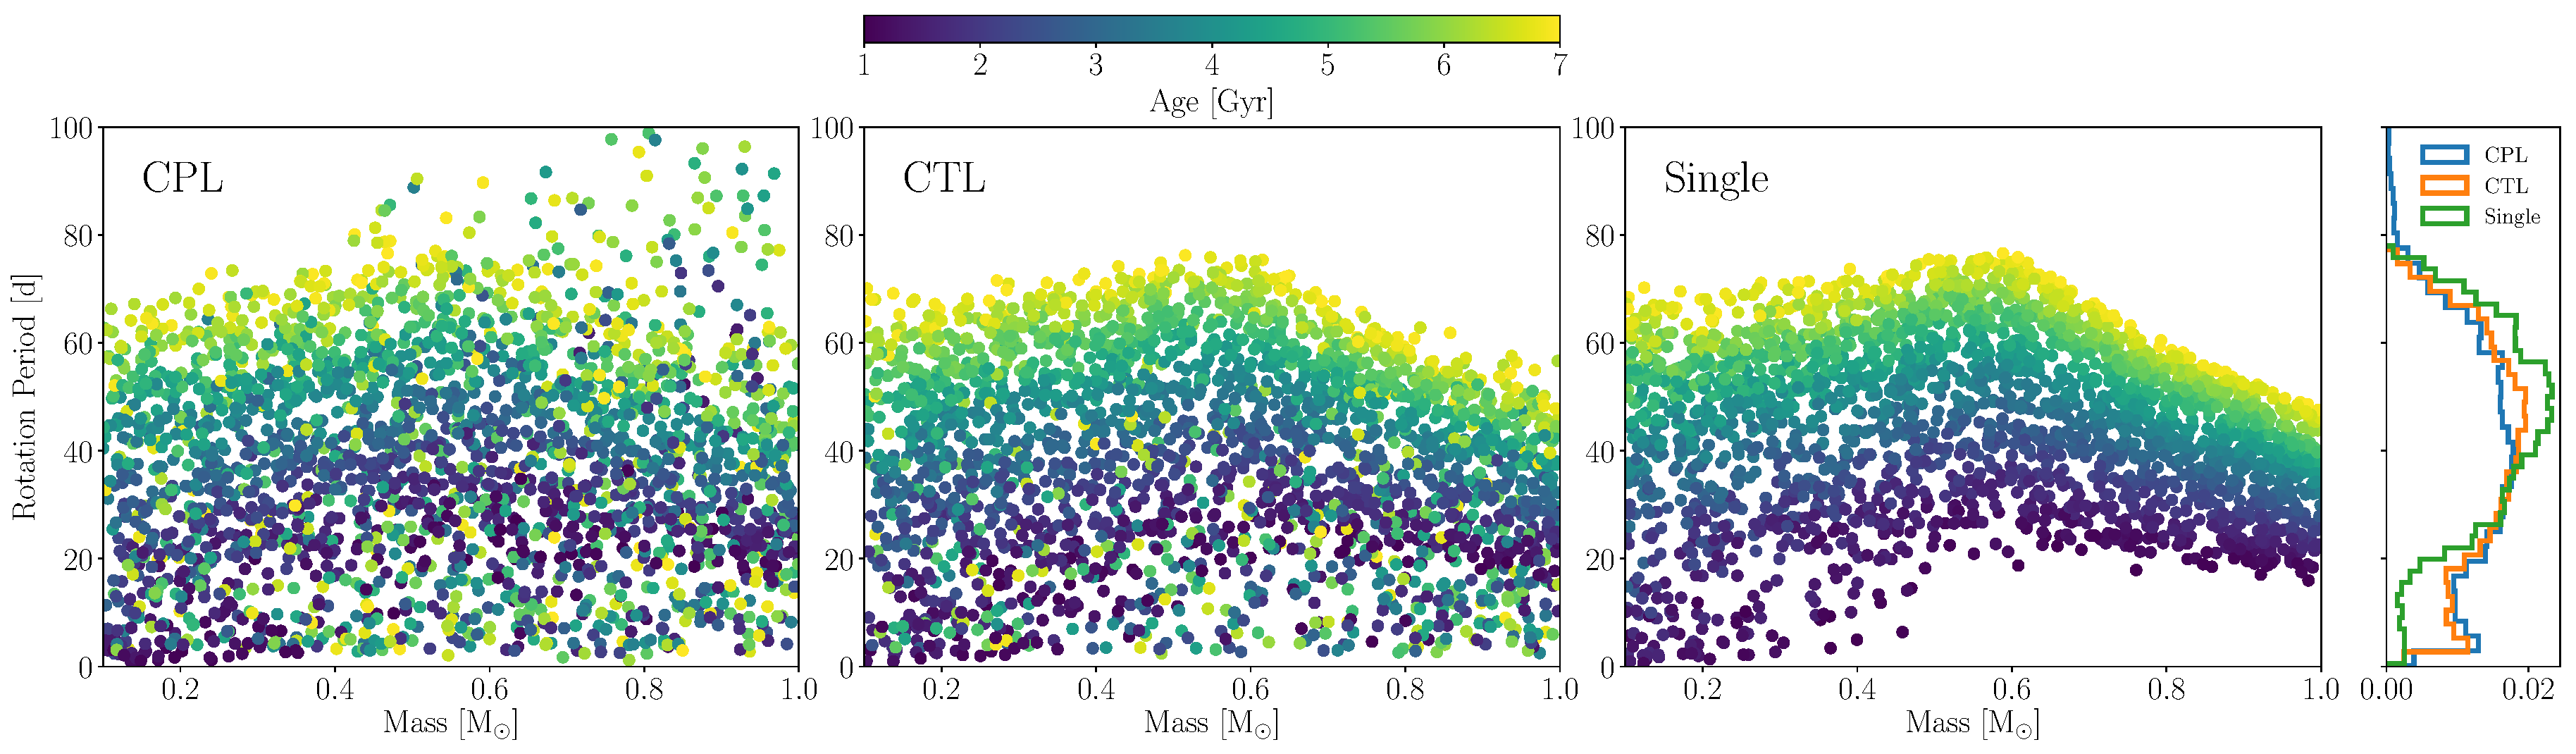
\includegraphics[width=\textwidth]{../Plots/protDist.pdf}
   \caption{P$_{rot}$ as a function of stellar mass and age according to our CPL (left), CTL (left center), and single star (right center) simulations. The P$_{rot}$ distribution for each case, marginalized over stellar mass, is depicted in the right panel. For each case, we only plot 2,500 systems for clarity but account for all systems when computing the marginalized distributions. Both tidal models predict a substantial population of fast rotators (P$_{rot} < 20$ d) not seen in the single star model at any age, except for young (age $< 2$ Gyr) M dwarfs (M$ < 0.5$ M$_{\odot}$). In many binary systems, both tidal models predict that age does not directly correlate with P$_{rot}$, especially in short P$_{orb}$ binaries where tidal torques are stronger, compared to the clear age-dependence of P$_{rot}$ seen in the single star models, the key assumption of gyrochronology methods.}%
    \label{fig:protDist}%
\end{figure*}

XXX

%% SECTION: COMPARISON TO KEPLER %%
\section{Comparison to \kepler} \label{sec:kepler}

XXX

\begin{figure*}[t]
	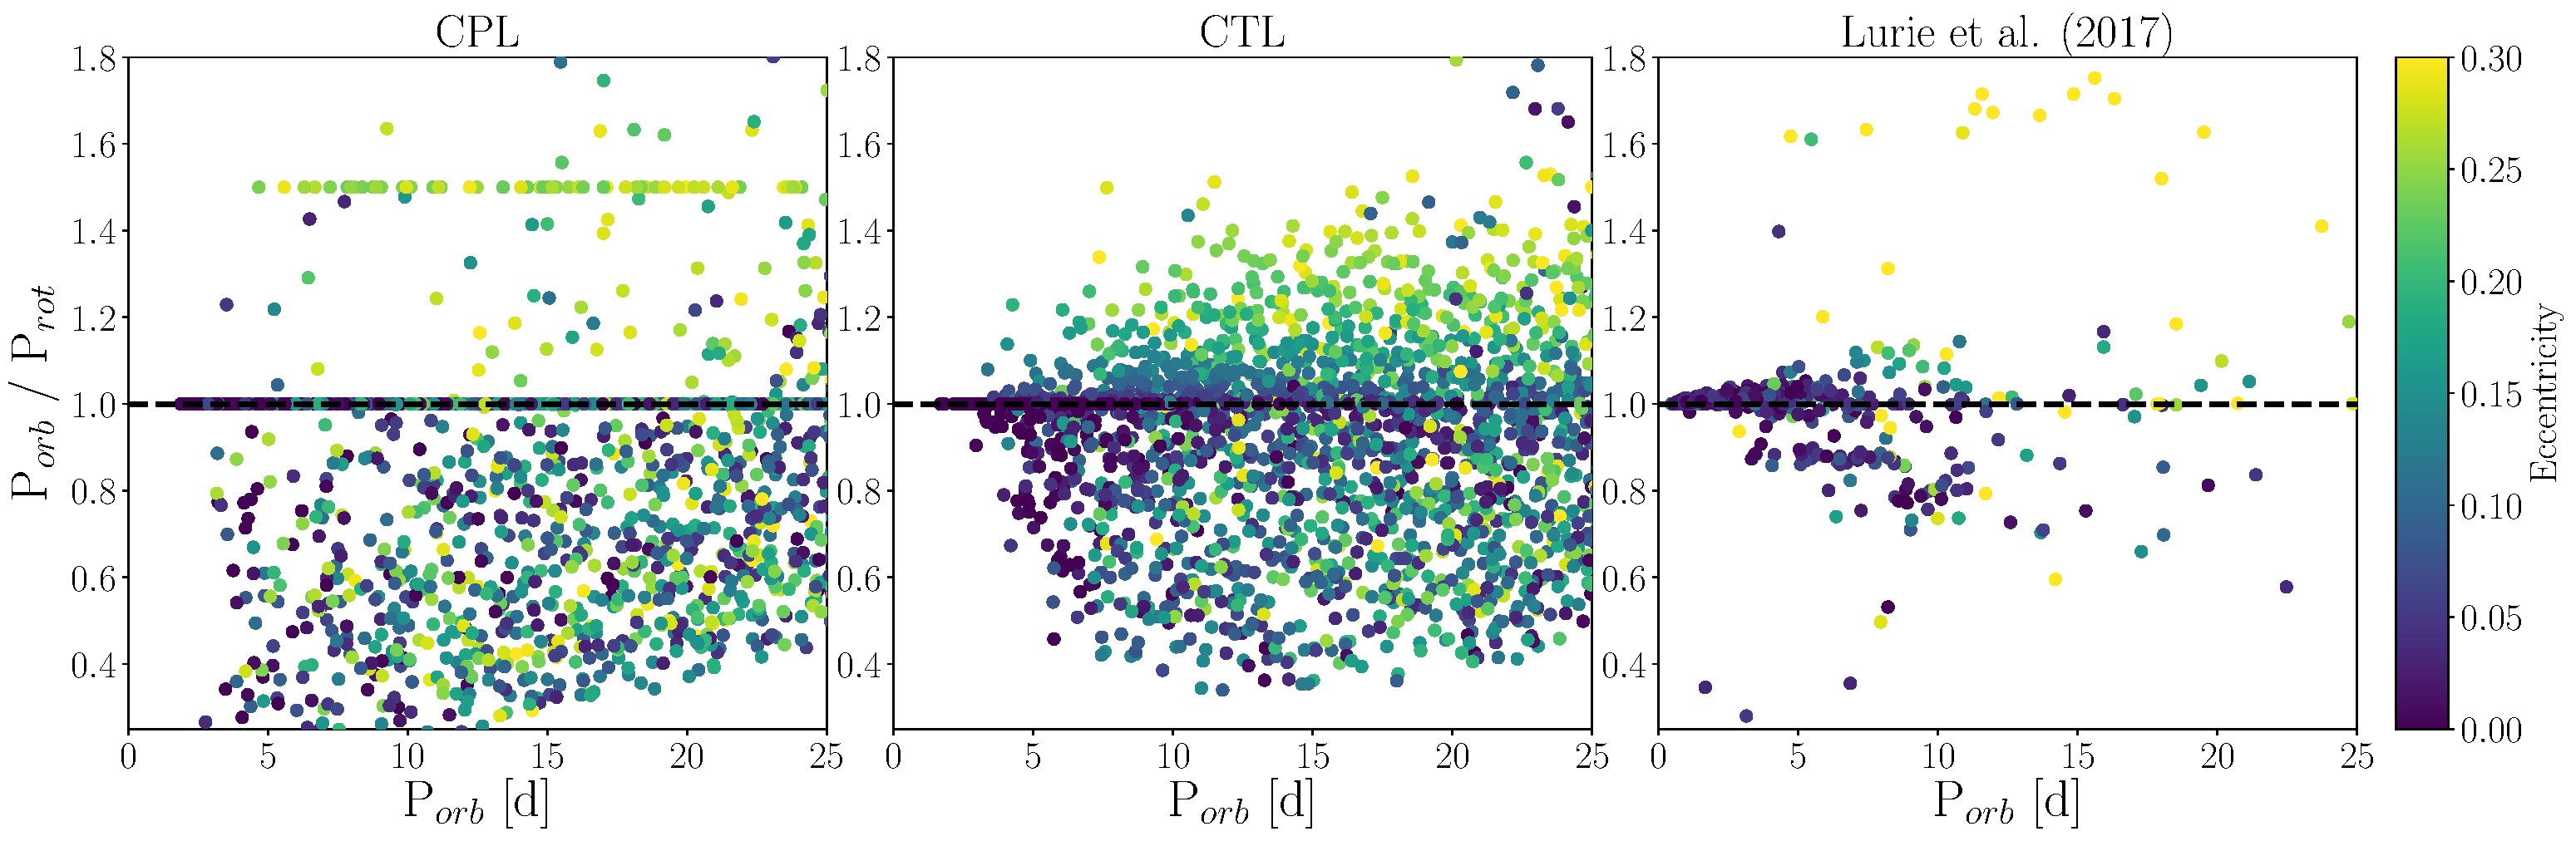
\includegraphics[width=\textwidth]{../Plots/lurieFig7.pdf}
   \caption{Caption}%
    \label{fig:lurie7}%
\end{figure*}

XXX

\subsection{P$_{orb} < 10$ d: The Subsynchronous Population} \label{sec:subsync}

XXX

\begin{figure}
	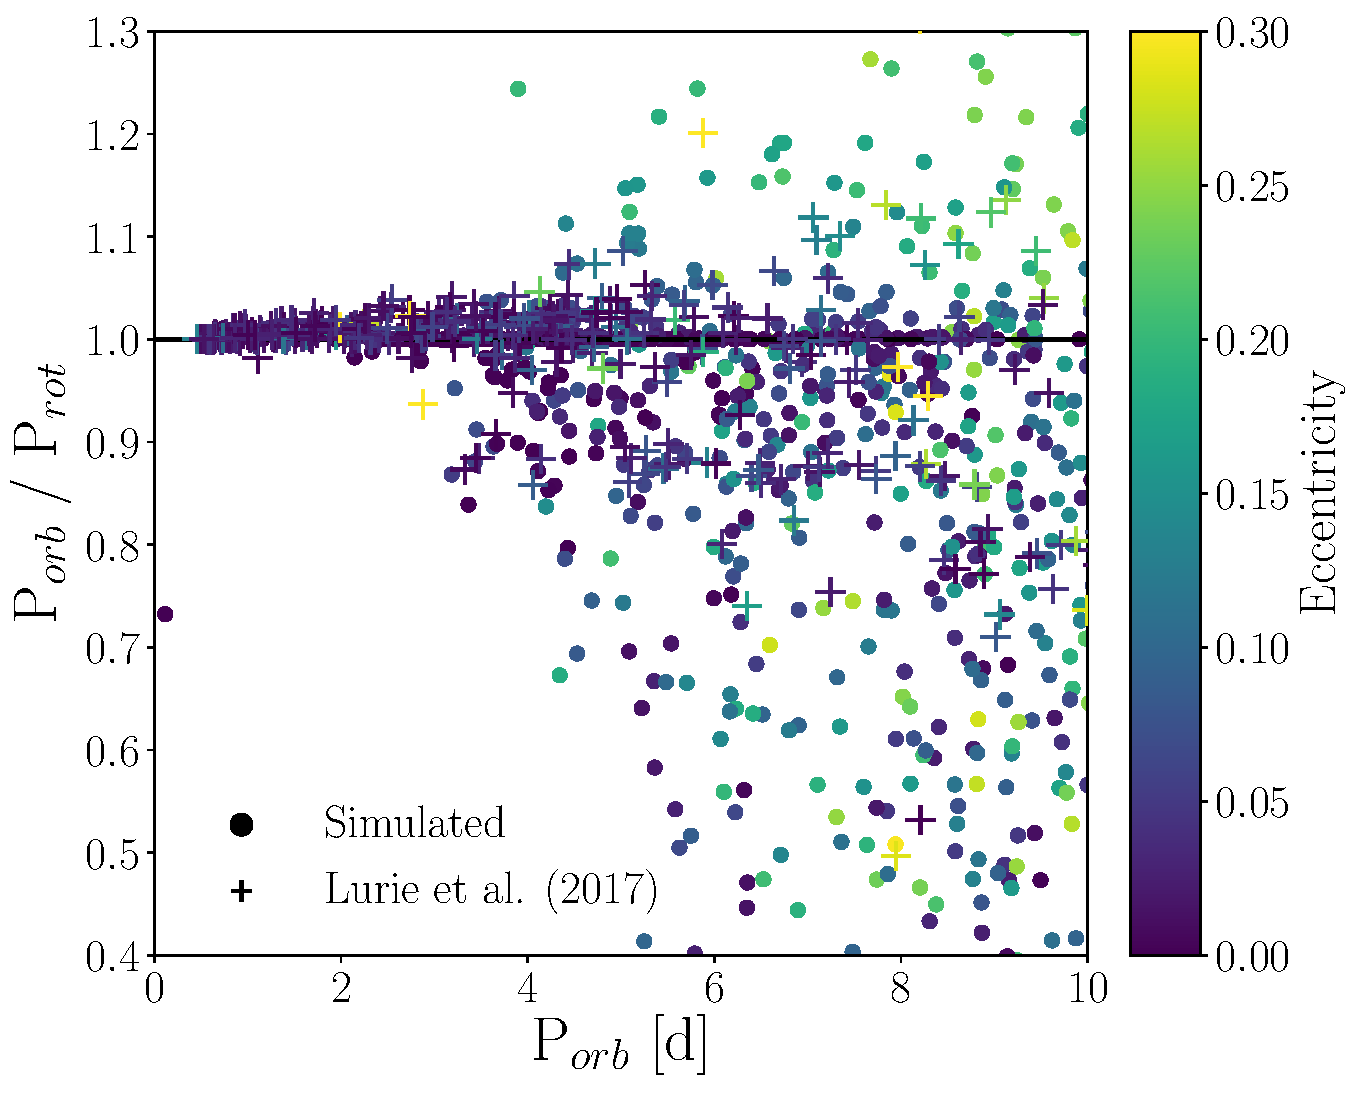
\includegraphics[width=0.45\textwidth]{../Plots/subsync.pdf}
   \caption{Caption}%
    \label{fig:subsync}%
\end{figure}

\subsection{$Q$, $\tau$ Constraints from P$_{orb}$ and P$_{rot}$} \label{sec:qTau}

\begin{figure}
	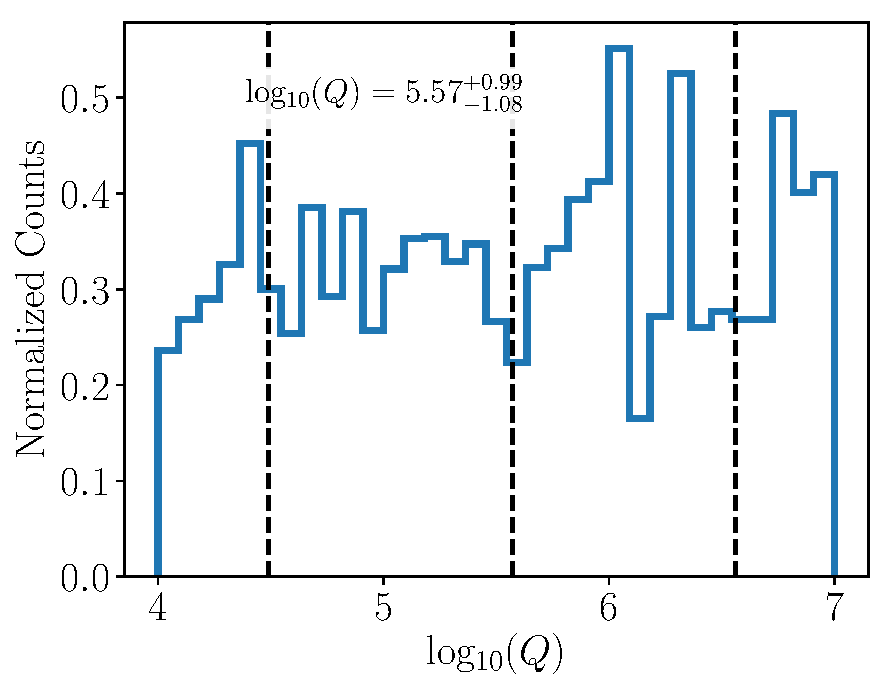
\includegraphics[width=0.45\textwidth]{../Plots/qLurie.pdf}
   \caption{Caption}%
    \label{fig:qLurie}%
\end{figure}

\begin{figure}
	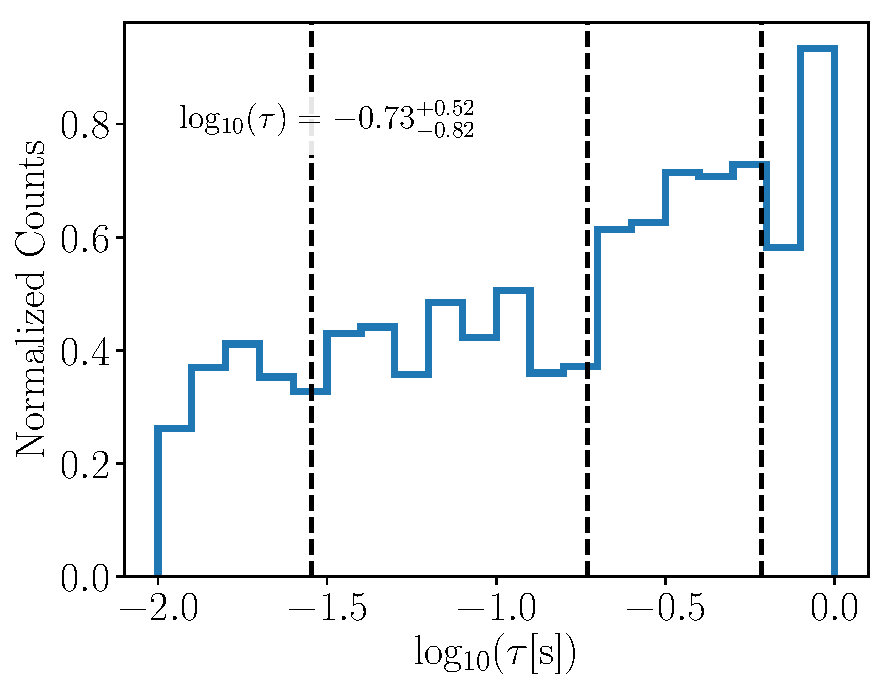
\includegraphics[width=0.45\textwidth]{../Plots/tauLurie.pdf}
   \caption{Caption}%
    \label{fig:tauLurie}%
\end{figure}

%% SECTION: DISCUSSION %%
\section{Discussion} \label{sec:discussion}

XXX

%% ACKNOWLEDGEMENTS %%
\acknowledgments
This work was facilitated though the use of advanced computational, storage, and networking infrastructure provided by the Hyak supercomputer system and funded by the STF at the University of Washington. This work was supported by NASA Headquarters under the NASA Earth and Space Science Fellowship Program - Grant 80NSSC17K0482.  DPF and RB acknowledge that this work was supported by the NASA Astrobiology Institute's Virtual Planetary Laboratory under Cooperative Agreement number NNA13AA93A. 

%% SOFTWARE %%
%\software{matplotlib: \citet{Hunter2007}, numpy: \citet{vanderWalt2011}, pandas: \citet{Mckinney2010}}

%% BIBLIOGRAPHY %%
\bibliography{sync}

\end{document}

%% End document %%
